%% Packages initialisation
\documentclass[10pt,compress]{beamer}
\usepackage[utf8]{inputenc}               % Enable UTF-8 compatible typing
\usepackage{hyperref}                     % Interactive PDF
\usepackage{listings}
\usepackage{xcolor}
\usepackage{multirow}
\usepackage{amssymb,mathtools}       % For mathematical writing
\usepackage{tikz}                    % Drawing trees
\usetikzlibrary{trees,shapes.multipart}
\usepackage[round]{natbib}
\usepackage[usenames,dvipsnames]{pstricks}
%\usepackage{epsfig}
\usepackage{pst-grad} % For gradients
\usepackage{pst-plot} % For axes

%% Use the default theme
\usetheme{default}

%% Colours block environment headings
\useinnertheme{rectangles}
\mode<beamer>{\setbeamertemplate{blocks}[rounded][shadow=false]} 
\setbeamercolor{block title}{bg=blue!10,fg=black}
\makeatletter
\pgfdeclareverticalshading[lower.bg,upper.bg]{bmb@transition}{200cm}{%
  color(0pt)=(upper.bg); color(2pt)=(upper.bg); color(4pt)=(upper.bg)}
\makeatother

%% Enable slide numbering
\makeatletter
\setbeamertemplate{footline}
{
  \leavevmode%
  \hbox{%
  \begin{beamercolorbox}[wd=.3\paperwidth,ht=2.25ex,dp=1ex,left]{author in head/foot}%
    \hspace*{2ex}\usebeamerfont{author in head/foot}\insertshortauthor~~\beamer@ifempty{\insertshortinstitute}{}{(\insertshortinstitute)}
  \end{beamercolorbox}%
  \begin{beamercolorbox}[wd=.5\paperwidth,ht=2.25ex,dp=1ex,center]{title in head/foot}%
    \usebeamerfont{title in head/foot}\insertshorttitle
  \end{beamercolorbox}%
  \begin{beamercolorbox}[wd=.1\paperwidth,ht=2.25ex,dp=1ex,center]{date in head/foot}%
    \usebeamerfont{date in head/foot}\insertshortdate{}
  \end{beamercolorbox}
  \begin{beamercolorbox}[wd=.1\paperwidth,ht=2.25ex,dp=1ex,right]{date in head/foot}%
    \usebeamerfont{date in head/foot}\insertframenumber /\inserttotalframenumber\hspace*{2ex}
  \end{beamercolorbox}}%
  \vskip0pt%
}
\makeatother

%% Hide navigation buttons
\beamertemplatenavigationsymbolsempty

%% Lstlisting style
\lstset{
 backgroundcolor=\color{white},   % choose the background color; you must add \usepackage{color} or \usepackage{xcolor}
 basicstyle=\ttfamily\footnotesize,        % the size of the fonts that are used for the code
 keywordstyle=\bfseries,
 commentstyle=\itshape,
 % SL: lstinline doesn't work properly if breakatwhitespace is not set to true
 breakatwhitespace=true,         % sets if automatic breaks should only happen at whitespace
 breaklines=true,                 % sets automatic line breaking
 captionpos=b,                    % sets the caption-position to bottom
 escapeinside={\#*}{*\#},          % if you want to add LaTeX within your code
 extendedchars=true,              % lets you use non-ASCII characters; for 8-bits encodings only, does not work with UTF-8
 frame=none,	                   % adds a frame around the code
 keepspaces=true,                 % keeps spaces in text, useful for keeping indentation of code (possibly needs columns=flexible)
 numbers=none,                    % where to put the line-numbers; possible values are (none, left, right)
 rulecolor=\color{black},         % if not set, the frame-color may be changed on line-breaks within not-black text (e.g. comments (green here))
 showspaces=false,                % show spaces everywhere adding particular underscores; it overrides 'showstringspaces'
 showstringspaces=false,          % underline spaces within strings only
 showtabs=false,                  % show tabs within strings adding particular underscores
 tabsize=1,	                   % sets default tabsize to 2 spaces
 title=\lstname,                   % show the filename of files included with \lstinputlisting; also try caption instead of title
 caption={},
 belowcaptionskip=-1\baselineskip,
 xleftmargin=0.1\parindent,
 columns=fullflexible
}

\lstdefinelanguage{Links}{% 
  morekeywords={typename, fun, op, var, if, this, true, false, else, case, switch, handle, handler, shallowhandler, open, do, sig},%
  sensitive=t, % 
  keywordstyle=\color{red},
  emph={Fail,Choose,Return},
  emphstyle={\color{blue}},
  comment=[l]{\#},% 
  escapeinside={(*}{*)},%
  morestring=[d]{"}%
 }

\newcommand{\textapprox}{{\fontfamily{ptm}\selectfont\texttildelow}}
\newcommand{\wildarrow}{\linksify{\textapprox{}>}}
% Links style
\lstdefinestyle{links}{
  basicstyle=\linespread{1.0}\ttfamily\footnotesize,
  language=Links,
  literate= {~>}{{\wildarrow}}1
}

\lstset{style={links}}

%% Checkmark
\def\checkmark{\tikz\fill[scale=0.4](0,.35) -- (.25,0) -- (1,.7) -- (.25,.15) -- cycle;}

%% Meta information
\author[Daniel Hillerström]{Daniel Hillerström\\\footnotesize{\href{mailto:daniel.hillerstrom@ed.ac.uk}{daniel.hillerstrom@ed.ac.uk}}\\\href{http://homepages.inf.ed.ac.uk/s1467124}{http://homepages.inf.ed.ac.uk/s1467124}}
\title{Compilation of Affine Algebraic Effect Handlers}
\subtitle{Master by Research intermediate progress review}
\institute{The University of Edinburgh}
\date{\today}

%% Slides
\begin{document}
% Front slide
\begin{frame}[plain]
  \maketitle
\end{frame}

\begin{frame}
  \frametitle{Recap story: Schedulers}
  Conventional programming languages implementations bake schedulers into the run-time system.
  
(c.f. \citet{Planas2009}, \citet{Augonnet2011} \citet{Openacc2013}, \citet{Openmp2013})
\vfill
  Best scheduling strategy is domain-specific (c.f. \citet{Dolan2015}):
  \begin{description}
    \item[Web-server] FIFO scheduling
    \item[Parallel search] LIFO work stealing
    \item[Data parallel] Gang scheduling
  \end{description}
  Claim: Effect handlers let us describe schedulers in the host language.
\end{frame}

% \begin{frame}
%   \frametitle{Programs are effectful}
% Virtually, every program comprise an \alert<1->{effectful} component, e.g.
% \begin{itemize}
%   \item raise exceptions
%   \item perform input/output
%   \item mutate some state
%   \item fork threads \uncover<2->{\alert<2->{$\Longleftarrow$ particular interested in modelling concurrency}}
%   \item non-determinism
%   \item \dots and so forth 
% \end{itemize}
% In most programming languages effects are dealt with \emph{implicitly}.

% Algebraic effects and handlers provide a modular abstraction for modelling and controlling effects \emph{explicitly}.
% \end{frame}

\begin{frame}
  \frametitle{Aims and objectives}
  Project overview
  \begin{description}
    \item[Phase 0] Write paper \checkmark
    \item[Phase 1] Compiler for Links with effect handlers \checkmark
    \item[Phase 2] Measure and implement optimisations for handlers
    \item[Phase 3] Message-passing concurrency via handlers
    \item[Phase 4] Message-passing parallelism via handlers
  \end{description}
\uncover<2->{Adding support for multicore parallelism ought to be ``free''.}
\end{frame}

\begin{frame}
  \frametitle{Infrastructure}
\begin{figure}
  \only<1-1>{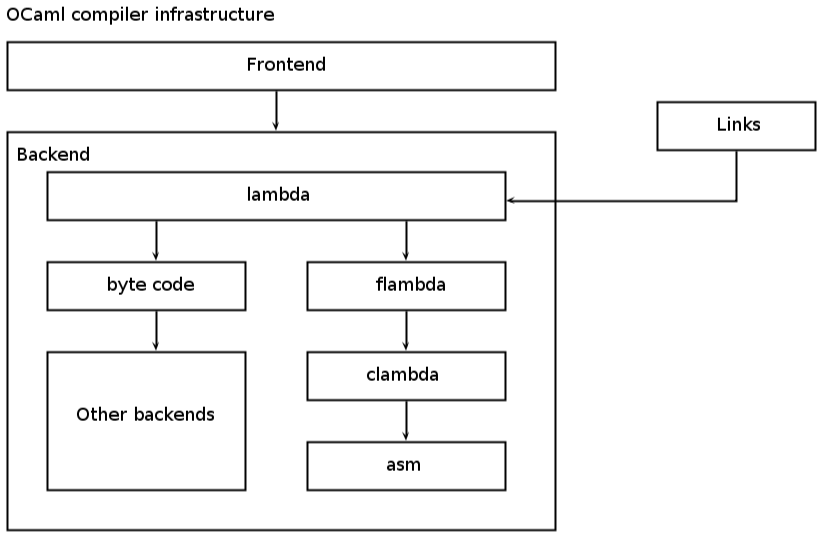
\includegraphics[scale=0.4]{infrastructure.png}}
  \only<2->{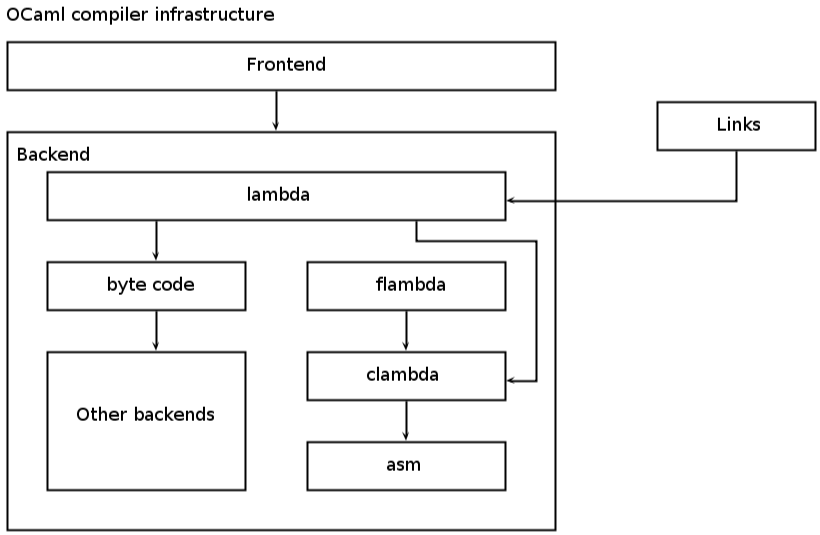
\includegraphics[scale=0.4]{infrastructure2.png}}
\end{figure}
\end{frame}

\begin{frame}
  \frametitle{Sanity checking}
  Microbenchmark: Pure counting (without handlers)
  \begin{table}
    \begin{tabular}{| l | r | r|}
      \hline
                  & Run-time (sec) & Speed up \\
      \hline
      Interpreter & 14.184         & 1.00 \\
      \hline
      Compiler    & 0.008          & 1773.00 \\
      \hline
    \end{tabular}
  \end{table}

  Microbenchmark: Stateful counting (using handlers)
  \begin{table}
    \begin{tabular}{| l | r | r|}
      \hline
                  & Run-time (sec) & Speed up \\
      \hline
      Interpreter & 76.884         & 1.00 \\
      \hline
      Compiler    & 1.644          & 46.77 \\
      \hline
    \end{tabular}
  \end{table}

\end{frame}

\begin{frame}
  \frametitle{Compiler demonstration}
  \begin{center}
    {\Huge\textbf{Demo}}
  \end{center}
\end{frame}

\begin{frame}
  \frametitle{Todo}
  Immediate future
  \begin{itemize}
    \item Pass exam\dots
    \item Set-up benchmarks -- fix compiler ``bugs''.
  \end{itemize}
  Near future
  \begin{itemize}
    \item Measure and implement optimisations.   
    \item Rebuild Links' message-passing concurrency model.
  \end{itemize}
  July-ish
  \begin{itemize}
    \item Begin focused write-up.
    \item Possibly add multicore support.
  \end{itemize}
\end{frame}

% Bibliography
\begin{frame}
  \frametitle{References}
  \bibliographystyle{abbrvnat}
  \bibliography{references}
\end{frame}
\end{document}